% =============================================================
%  Tầm nhìn & Mục tiêu chi tiết
%  Vision & Objectives — calibrated to 2026 trends + team capabilities
%  Đà Nẵng, 2026
%  Biên dịch: xelatex tam-nhin-muc-tieu.tex
% =============================================================
\documentclass[11pt,a4paper]{article}

\usepackage[margin=2.2cm,top=2cm,bottom=2.2cm]{geometry}
\usepackage{fontspec}
\usepackage{tikz}
\usepackage{xcolor}
\usepackage{tabularx}
\usepackage{booktabs}
\usepackage{enumitem}
\usepackage{titlesec}
\usepackage{fancyhdr}
\usepackage{hyperref}
\usepackage{setspace}
\usepackage{tcolorbox}
\usepackage{amssymb}
\tcbuselibrary{skins, breakable}
\usetikzlibrary{positioning, shapes.geometric, shapes.misc, arrows.meta,
                fit, calc, decorations.pathreplacing, backgrounds, chains}

\setmainfont{Latin Modern Roman}
\setsansfont{Latin Modern Sans}

\definecolor{ink}{HTML}{14213d}
\definecolor{accent}{HTML}{fca311}
\definecolor{mid}{HTML}{8d99ae}
\definecolor{ok}{HTML}{2a9d8f}
\definecolor{warn}{HTML}{c44536}
\definecolor{soft}{HTML}{f4f1de}
\definecolor{leaf}{HTML}{3d5a80}
\definecolor{cool}{HTML}{5e6472}
\definecolor{vision}{HTML}{1d3557}
\definecolor{ambition}{HTML}{e07a5f}
\definecolor{capacity}{HTML}{457b9d}

\hypersetup{colorlinks=true, linkcolor=ink, urlcolor=leaf}

\titleformat{\section}{\sffamily\bfseries\LARGE\color{ink}}{Chương \thesection.}{0.5em}{}
\titleformat{\subsection}{\sffamily\bfseries\large\color{ink}}{\thesubsection}{0.5em}{}
\titleformat{\subsubsection}{\sffamily\bfseries\normalsize\color{ink}}{}{0em}{}
\titlespacing*{\section}{0pt}{1.4em}{0.6em}
\titlespacing*{\subsection}{0pt}{1.0em}{0.3em}
\titlespacing*{\subsubsection}{0pt}{0.6em}{0.2em}

\setlist{nosep, leftmargin=1.3em, topsep=3pt, itemsep=2pt}
\setlength{\parskip}{4pt}
\setlength{\parindent}{0pt}
\onehalfspacing

\pagestyle{fancy}
\fancyhf{}
\fancyhead[L]{\sffamily\footnotesize\color{mid} Tầm nhìn \& Mục tiêu}
\fancyhead[R]{\sffamily\footnotesize\color{mid} Internal \textbullet{} 2026}
\fancyfoot[C]{\sffamily\footnotesize\color{mid}\thepage}
\renewcommand{\headrulewidth}{0pt}

\newtcolorbox{keybox}[1][]{
  enhanced, colback=soft, colframe=accent, boxrule=0.5pt,
  left=8pt, right=8pt, top=5pt, bottom=5pt, arc=1pt,
  fonttitle=\sffamily\bfseries\color{ink}, #1
}
\newtcolorbox{warnbox}[1][]{
  enhanced, colback=warn!8, colframe=warn, boxrule=0.5pt,
  left=8pt, right=8pt, top=5pt, bottom=5pt, arc=1pt,
  fonttitle=\sffamily\bfseries\color{warn}, #1
}
\newtcolorbox{visionbox}[1][]{
  enhanced, colback=vision!6, colframe=vision, boxrule=0.5pt,
  left=8pt, right=8pt, top=5pt, bottom=5pt, arc=1pt,
  fonttitle=\sffamily\bfseries\color{vision}, #1
}
\newtcolorbox{quotebox}[1][]{
  enhanced, colback=white, colframe=ink!30, boxrule=0pt,
  borderline west={2pt}{0pt}{ink},
  left=10pt, right=8pt, top=4pt, bottom=4pt, arc=0pt, #1
}

\begin{document}

% =============================================================
% TITLE PAGE
% =============================================================
\thispagestyle{empty}
\vspace*{3cm}
\begin{center}
{\sffamily\bfseries\fontsize{32}{38}\selectfont\color{ink} Tầm nhìn \& Mục tiêu}\\[0.5em]
{\sffamily\Large\color{mid} Vision \& Objectives}\\[0.5em]
{\sffamily\large\color{mid} University Quality OS \textbullet{} 2026--2036}\\[3em]

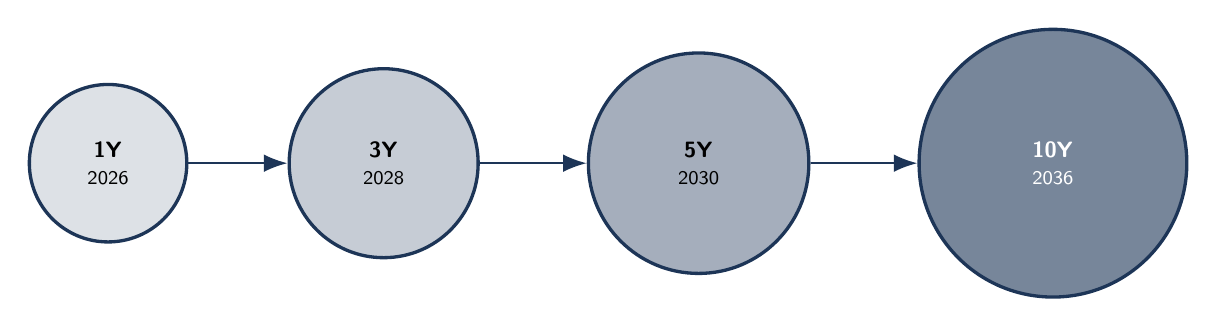
\begin{tikzpicture}[font=\sffamily\footnotesize]
  \node[circle, draw=vision, very thick, fill=vision!15, minimum size=2cm, align=center] (v1) at (0,0) {\textbf{1Y}\\\scriptsize 2026};
  \node[circle, draw=vision, very thick, fill=vision!25, minimum size=2.4cm, align=center] (v3) at (3.5,0) {\textbf{3Y}\\\scriptsize 2028};
  \node[circle, draw=vision, very thick, fill=vision!40, minimum size=2.8cm, align=center] (v5) at (7.5,0) {\textbf{5Y}\\\scriptsize 2030};
  \node[circle, draw=vision, very thick, fill=vision!60, minimum size=3.4cm, align=center, font=\sffamily\footnotesize\color{white}] (v10) at (12,0) {\textbf{10Y}\\\scriptsize 2036};

  \draw[-{Latex[length=3mm]}, thick, vision] (v1) -- (v3);
  \draw[-{Latex[length=3mm]}, thick, vision] (v3) -- (v5);
  \draw[-{Latex[length=3mm]}, thick, vision] (v5) -- (v10);
\end{tikzpicture}

\vspace{2em}
{\large\color{vision}\sffamily\itshape
``Hệ điều hành chất lượng cho đại học Đông Nam Á.''
}\\[3em]

{\sffamily\color{mid} Đà Nẵng, tháng 4 năm 2026}
\end{center}
\vfill
\begin{center}
{\footnotesize\itshape\color{mid}
Tài liệu này định nghĩa tầm nhìn dài hạn và mục tiêu cụ thể của\\
University Quality OS, được calibrate theo bối cảnh agentic AI 2026\\
và năng lực thực tế của team Hảo--Phú--Hoàng + CAIRA-DAU.\\
Nó là tài liệu nền tảng để mọi quyết định chiến lược tham chiếu lại.}
\end{center}
\clearpage

\tableofcontents
\clearpage

% =============================================================
% TÓM TẮT
% =============================================================
\section*{Tóm tắt --- Vision \& Objectives trên 1 trang}
\addcontentsline{toc}{section}{Tóm tắt --- Vision \& Objectives trên 1 trang}

\begin{visionbox}[title=Tầm nhìn 10 năm (2036)]
\textbf{Trở thành \textit{operating system} cho công tác đảm bảo chất lượng giáo dục
đại học tại Đông Nam Á} --- nơi mà khi một trường đại học muốn vận hành quy
trình ISO, tự đánh giá KĐCLGD, đo PLO/CLO, hoặc kết nối với khung quốc tế
(ABET, AUN-QA), tên chúng tôi là tên đầu tiên họ nghĩ đến.
\end{visionbox}

\textbf{4 mốc tầm nhìn:}

\begin{tabularx}{\linewidth}{@{}p{1.3cm} X X@{}}
\toprule
\textbf{Năm} & \textbf{Tầm nhìn ngắn} & \textbf{North Star metric} \\
\midrule
\textbf{2026} & CAIRA-DAU thành công, ship 2 use case agentic tại DAU & 1 hệ thống production tại DAU + 60 KPI CAIRA đạt $\geq$ 70\% \\
\textbf{2028} & Spin-out (nếu validate được) hoặc CAIRA mạnh, 3-5 trường VN dùng & 5+ trường, framework v2, 1 paper top-tier \\
\textbf{2030} & VN leader trong agentic AI cho giáo dục, mở rộng ĐNA & 30-50 khách, doanh thu 15-25 tỷ VND, 1-3 khách ĐNA \\
\textbf{2036} & ĐNA leader, có ảnh hưởng quốc tế trong vertical & 200+ tổ chức tri thức, 5+ quốc gia, IPO-able hoặc strategic acquisition \\
\bottomrule
\end{tabularx}

\textbf{5 mục tiêu xuyên suốt:}

\begin{enumerate}
\item \textbf{Sản phẩm:} University Quality OS — agentic layer kết nối ISO + KĐCLGD + PLO/CLO.
\item \textbf{Thị trường:} Giáo dục đại học Việt Nam → Đông Nam Á → các tổ chức tri thức khác.
\item \textbf{Thương hiệu:} ``Stripe của quality management cho ĐNA giáo dục'' --- chọn vì độ tin cậy hạ tầng, không phải vì tính năng.
\item \textbf{Năng lực:} Vertical depth (KĐCLGD + ISO + AI) + framework leverage + Vietnamese context by default.
\item \textbf{Tác động:} Giải phóng cán bộ giáo dục khỏi việc lặp lại, để họ làm việc con người nên làm.
\end{enumerate}

\textbf{3 nguyên tắc không thay đổi:}

\begin{itemize}
\item \textbf{CAIRA-first.} Mọi việc bắt đầu từ và quay về phục vụ CAIRA-DAU.
\item \textbf{Trust over hype.} Chọn citations + audit + governance trước tính năng wow.
\item \textbf{Asymmetric bet.} Floor cao (CAIRA thành công) + ceiling cao (spin-out scale ĐNA), không có catastrophic fail.
\end{itemize}

\clearpage

% =============================================================
% PART I — BỐI CẢNH 2026
% =============================================================
\begin{center}
\vspace*{0.5em}
{\sffamily\bfseries\Huge\color{ink} Phần I}\\[0.5em]
{\sffamily\LARGE\color{mid} Bối cảnh 2026}\\[0.5em]
{\color{ink}\rule{6cm}{0.4pt}}
\end{center}
\vspace{1em}

% =============================================================
\section{Bức tranh agentic AI toàn cầu \& Việt Nam (2026)}

\subsection{Agentic AI đã trưởng thành --- nhưng adoption vẫn ở đầu đường cong}

Sau 4 năm kể từ ChatGPT (cuối 2022), AI doanh nghiệp đã đi qua 3 pha:

\begin{tabularx}{\linewidth}{@{}p{2.5cm} p{2.5cm} X@{}}
\toprule
\textbf{Pha} & \textbf{Thời gian} & \textbf{Đặc điểm} \\
\midrule
\textbf{Chatbot} & 2023 & Q\&A đơn giản, ROI mơ hồ. ``AI gì cũng được'' đợt đầu. \\
\textbf{Copilot} & 2024 & Tích hợp vào tools sẵn (GitHub, Word, Notion). Bão hoà nhanh. \\
\textbf{Agentic} & 2025-2026 & AI \emph{tự làm} workflow có công cụ, có kiểm soát, có evals. \\
\textbf{Autonomous} & 2027+ & Agent quản lý agent. Còn xa, không phải hiện tại. \\
\bottomrule
\end{tabularx}

\textbf{Tín hiệu chín:}
\begin{itemize}
\item \textbf{Foundation models} đã ổn định: Claude 4.x với 1M context, tool use 99\%+ reliability, multimodal.
\item \textbf{Cost inference} giảm 50\% mỗi 6 tháng. Một query agent 2026 chi phí ~ \$0.01-0.05.
\item \textbf{Agentic frameworks} đã production-ready: Pydantic AI, LangGraph, Anthropic's Computer Use, OpenAI Agents SDK.
\item \textbf{Evaluation \& observability} (Langfuse, Braintrust, Weights \& Biases) đã chuẩn hoá.
\item \textbf{Anthropic + OpenAI + Google} công khai khuyến nghị bắt đầu từ workflow rõ + guardrails, lên multi-agent chỉ khi cần.
\end{itemize}

\subsection{Adoption thực tế: \textit{nói} nhiều, \textit{ship} ít}

\textbf{Số liệu thị trường global (Q4/2025):}
\begin{itemize}
\item McKinsey ước tính giá trị kinh tế từ agentic AI: \$4.4 nghìn tỷ USD/năm toàn cầu (lý thuyết).
\item Deloitte: 78\% lãnh đạo nói ``đã có chiến lược AI'', nhưng chỉ 12\% có ít nhất 1 hệ thống agentic chạy production.
\item BCG: 70\% thất bại của AI projects là do organizational + workflow design, không phải kỹ thuật.
\end{itemize}

\textbf{Hàm ý:} Cửa sổ ship-first vẫn mở. Người \textit{ship được production} trong 18-24 tháng tới chiếm vị thế 5-10 năm sau.

\subsection{Việt Nam: thị trường ``dưới ngưỡng'' đang dậy sóng}

Thị trường AI Việt Nam 2026:
\begin{itemize}
\item \textbf{Big tech VN} (FPT, VNG, CMC) tập trung tập đoàn lớn (ngân hàng, viễn thông, sản xuất).
\item \textbf{Startup AI VN} chủ yếu wrapper ChatGPT (chatbot tuyển sinh, customer service generic).
\item \textbf{Vertical sâu} (giáo dục, y tế, nông nghiệp) gần như chưa có ai làm production-grade agentic.
\item \textbf{Government push:} Đề án Chuyển đổi số quốc gia 2030 + Chiến lược AI 2030 + nhiều ngân sách dành cho ứng dụng AI.
\end{itemize}

\textbf{Hệ quả:} Vertical nào có ai \textit{hiểu cả công nghệ + ngành} bắt đầu trước, sẽ ít cạnh tranh trong 24-36 tháng tới. Đây chính xác là cửa sổ chúng tôi đang nhắm.

\subsection{Cụ thể: Agentic AI cho giáo dục đại học Việt Nam}

Khảo sát nhanh 2026 (theo network của Hảo + nguồn công khai):

\begin{tabularx}{\linewidth}{@{}p{4.5cm} X@{}}
\toprule
\textbf{Loại player} & \textbf{Trạng thái 2026} \\
\midrule
Big tech (OpenAI, Anthropic, Google) & Chưa ưu tiên VN giáo dục (TAM nhỏ, locale phức tạp). \\
FPT.AI / VNG / VinAI & Cung cấp platform chung; chưa ship vertical solution cho trường ĐH. \\
EduTech VN (VioEdu, Marathon, Topica) & Tập trung học sinh, không phải vận hành nhà trường. \\
Chatbot tuyển sinh (vài startup nhỏ) & Câu trả lời tự động đơn giản; không phải agentic. \\
Trường ĐH tự xây & Một vài trường có lab AI nhưng không scale. CAIRA-DAU là pioneer. \\
\bottomrule
\end{tabularx}

\textbf{Kết luận:} Phân khúc \textit{agentic AI cho công tác đảm bảo chất lượng + vận hành đại học} là \textbf{open white space}. Người vào trước với chất lượng production có thể chiếm 5-10\% thị trường VN trong 3-5 năm.

\clearpage

% =============================================================
\section{Giáo dục Việt Nam đang chuyển mình}

\subsection{3 lực đẩy chính 2026-2030}

\subsubsection*{1. Áp lực kiểm định chất lượng (mới + chặt hơn)}

\textbf{Thông tư 2026/TT-BGDĐT} (vừa ban hành) định nghĩa khung KĐCLGD mới:
\begin{itemize}
\item 15 tiêu chuẩn / 60 tiêu chí (chi tiết hơn TT 2024)
\item Hướng outcome-based: nhấn mạnh \textit{kết quả đào tạo}, không chỉ \textit{quy trình}
\item Chu kỳ TĐG: 5 năm/lần, mỗi lần ngốn 6 tháng × 10 người của một trường
\item Bắt buộc với mọi trường ĐH muốn duy trì hoạt động hợp pháp
\end{itemize}

\textbf{Hàm ý:} 240 trường ĐH VN đều có pain point này. Chi phí thuê consultant: 500M-2B VND/chu kỳ. Tổng TAM riêng KĐCLGD ~ 60-200 tỷ/năm.

\subsubsection*{2. Áp lực chuẩn quốc tế (ABET, AUN-QA)}

\begin{itemize}
\item Top 30 trường VN đang theo đuổi AUN-QA (chuẩn ASEAN University Network).
\item Top 10 đang/sẽ theo đuổi ABET (chuẩn engineering của Mỹ).
\item Cả 2 đều yêu cầu đo PLO/CLO chặt chẽ, có evidence chain.
\item Hiện tại: 95\% trường làm thủ công bằng Excel.
\end{itemize}

\subsubsection*{3. Áp lực chuyển đổi số (mandate quốc gia)}

\begin{itemize}
\item Chính phủ ban hành \textbf{Chương trình Chuyển đổi số Giáo dục 2026-2030}: bắt buộc trường ĐH có hệ thống quản lý số hoá toàn diện.
\item Ngân sách hỗ trợ: 5-10\% trong tổng ngân sách CNTT của trường được khuyến khích cho AI.
\item Hiệu trưởng/HĐT chịu trách nhiệm direct về tiến độ.
\end{itemize}

\subsection{Buyer behavior \& willingness to pay}

\textbf{Profile khách hàng giáo dục VN (qua discovery sơ bộ + network Hảo):}

\begin{tabularx}{\linewidth}{@{}p{4cm} X@{}}
\toprule
\textbf{Đặc điểm} & \textbf{Hàm ý} \\
\midrule
Ngân sách CNTT 500M-3B/năm/trường & Đủ chi cho AI nếu ROI rõ \\
Chu kỳ ra quyết định 2-4 tháng & Sales motion phải patient + relationship-driven \\
Sợ ``AI ảo'' và data leak & Phải có citations + audit trail + on-prem option \\
Tin academic peers > vendors & PhD-to-PhD warm intro hiệu quả 10$\times$ cold outreach \\
Chu kỳ mua lớn nhất: tháng 1-2, 6-7 (sau học kỳ) & Time GTM theo academic calendar \\
\bottomrule
\end{tabularx}

\textbf{Willingness to pay (ước):}
\begin{itemize}
\item 50-150 triệu VND cho pilot 2-3 tháng (10-15\% ngân sách CNTT)
\item 200-500 triệu VND/năm cho solution + ops (sau pilot)
\item 1-3 tỷ VND cho deployment lớn (AUN-QA, ABET prep)
\end{itemize}

\subsection{Vì sao Việt Nam đặc biệt phù hợp với chúng tôi}

\begin{enumerate}
\item \textbf{Local expertise required:} Nội dung tiếng Việt, văn bản BGDĐT, quy chế trường --- big tech khó.
\item \textbf{Network academic của Hảo} là tài sản hiếm: PhD VN có quan hệ với nhiều trường = warm intros.
\item \textbf{Chi phí vận hành thấp:} ĐN 1 engineer = 1/3 chi phí Hà Nội/HCM.
\item \textbf{ĐNA expansion path:} Workflow giáo dục VN tương tự PH/ID/TH --- có thể export.
\item \textbf{Chính phủ ủng hộ:} Mandate transformation = no political headwind.
\end{enumerate}

\clearpage

% =============================================================
\section{Cửa sổ thời gian \& Why now}

\subsection{Cửa sổ là 2026-2028}

\begin{center}
\begin{tikzpicture}[font=\sffamily, scale=0.95]
  % Timeline
  \draw[ink!50, very thick] (0,0) -- (15,0);
  \foreach \x/\m in {0/2024, 3/2026, 6/2028, 9/2030, 12/2032, 15/2034} {
    \draw[ink!50, thick] (\x,0.15) -- (\x,-0.15);
    \node[below=1mm, font=\footnotesize] at (\x,-0.15) {\m};
  }

  % Phases
  \draw[decorate, decoration={brace, amplitude=5pt}, ok, ultra thick] (3,0.5) -- (6,0.5)
    node[midway, above=5pt, font=\sffamily\bfseries\small, ok] {VINDOW: build position};
  \draw[decorate, decoration={brace, amplitude=5pt}, accent, thick] (6,0.5) -- (9,0.5)
    node[midway, above=5pt, font=\sffamily\bfseries\small, accent] {Defend + scale};
  \draw[decorate, decoration={brace, amplitude=5pt}, mid, thick] (9,0.5) -- (15,0.5)
    node[midway, above=5pt, font=\sffamily\small, mid] {Mature market, harder to enter};

  % Events
  \node[font=\tiny\sffamily, ink, align=center, text width=2.5cm] at (3,-1) {TT 2026 BGDĐT\\hiệu lực};
  \node[font=\tiny\sffamily, ink, align=center, text width=2.5cm] at (6,-1) {Ước: big tech\\bắt đầu để ý VN};
  \node[font=\tiny\sffamily, ink, align=center, text width=2.5cm] at (9,-1) {Ước: 5-10 player\\trong vertical};
  \node[font=\tiny\sffamily, ink, align=center, text width=2.5cm] at (12,-1) {Vertical leader\\đã định hình};
\end{tikzpicture}
\end{center}

Cửa sổ \textbf{18-30 tháng} (2026 Q2 → 2028 Q4) để xác lập vị thế first-shipper. Sau đó:

\begin{itemize}
\item \textbf{Big tech VN} (FPT, VNG) sẽ launch competitor sau khi thấy thị trường rõ.
\item \textbf{Startup mới} sẽ vào sau 12-18 tháng.
\item \textbf{Khách hàng đầu} đã lock-in với ai đó --- switching cost đẩy họ ở lại.
\end{itemize}

\subsection{Why now --- 7 lý do}

\begin{enumerate}
\item \textbf{Công nghệ vừa đủ chín.} Claude 4.x, Pydantic AI, pgvector --- ship được production.
\item \textbf{Cost inference đủ thấp} cho B2B mid-market VN trả nổi.
\item \textbf{Mandate KĐCLGD mới} (TT 2026) tạo urgency cho 240 trường.
\item \textbf{CAIRA-DAU vừa thành lập} (Hảo bổ nhiệm 17/4/2026) --- mandate official, ngân sách có.
\item \textbf{Cửa sổ chưa có competitor} mạnh trong vertical này tại VN.
\item \textbf{Chi phí cá nhân thấp:} CAIRA budget cover, founders không phải bỏ tiền lớn.
\item \textbf{Network của Hảo trong giáo dục} đang ở đỉnh điểm hữu dụng nhất.
\end{enumerate}

\subsection{Why us --- 5 lý do}

\begin{enumerate}
\item \textbf{Hảo có 4 thứ hiếm cùng lúc:} PhD telecoms (kỹ thuật), giảng viên DAU (network), CAIRA Director (mandate), kinh nghiệm KĐCLGD/CTĐT (domain).
\item \textbf{Phú đã làm việc với Hảo} --- không phải build trust từ đầu, có thể start ngay.
\item \textbf{Hoàng có business background} bù phần còn thiếu của 2 người academic.
\item \textbf{DAU là institutional shelter} --- 12-18 tháng được trả lương để R\&D, hiếm có.
\item \textbf{Đà Nẵng location} --- chi phí thấp + hệ sinh thái tech + không phải cạnh tranh tuyển dụng với HN/HCM.
\end{enumerate}

\clearpage

% =============================================================
% PART II — TẦM NHÌN
% =============================================================
\begin{center}
\vspace*{0.5em}
{\sffamily\bfseries\Huge\color{vision} Phần II}\\[0.5em]
{\sffamily\LARGE\color{mid} Tầm nhìn theo mốc thời gian}\\[0.5em]
{\color{vision}\rule{6cm}{0.4pt}}
\end{center}
\vspace{1em}

% =============================================================
\section{Tầm nhìn 10 năm (2036)}

\subsection{Phát biểu tầm nhìn}

\begin{visionbox}[title=Tầm nhìn 2036]
\textbf{University Quality OS là hệ điều hành chuẩn cho công tác đảm bảo chất
lượng và vận hành đại học tại Đông Nam Á.}

Khi một trường đại học, một viện nghiên cứu, hoặc một tổ chức đào tạo trong
khu vực --- từ Manila đến Jakarta đến Bangkok đến Hà Nội --- bắt đầu suy nghĩ
về việc \textit{tự động hóa quy trình tri thức một cách an toàn và có kiểm
soát}, tên đầu tiên họ nghĩ đến là chúng tôi.
\end{visionbox}

\subsection{Bức tranh cụ thể 2036}

\subsubsection*{Quy mô}
\begin{itemize}
\item \textbf{Khách hàng:} 200-300 tổ chức tri thức, trong đó 100+ ở Việt Nam (chiếm 40\% thị trường VN), 100+ phân bố Philippines, Indonesia, Thailand, Malaysia, Singapore.
\item \textbf{Doanh thu:} 200-500 tỷ VND/năm (8-20 triệu USD).
\item \textbf{ARR (subscription):} 70\%+ tổng doanh thu.
\item \textbf{Nhân sự:} 100-150 người, văn phòng tại Đà Nẵng + 2-3 hub khác (Manila, Jakarta, Bangkok).
\item \textbf{Profitable:} Operating margin 15-25\%, không phụ thuộc next funding round.
\end{itemize}

\subsubsection*{Sản phẩm}
\begin{itemize}
\item \textbf{Quality OS Core:} Suite chuẩn cho mọi trường: Admissions, Internal Knowledge, Quality Assurance, Curriculum, Research Support.
\item \textbf{Industry verticals:} Mở rộng sang viện nghiên cứu, hội đồng kiểm định khu vực, tổ chức đào tạo doanh nghiệp.
\item \textbf{API platform:} EdTech khác có thể build trên top our platform (developer ecosystem 100+ apps).
\item \textbf{Compliance hub:} Tích hợp mọi chuẩn (KĐCLGD VN, AUN-QA, ABET, WASC, EQUIS).
\end{itemize}

\subsubsection*{Thương hiệu}
\begin{itemize}
\item \textbf{Top-3 ĐNA} về AI cho giáo dục đại học (theo các báo cáo Frost \& Sullivan, IDC).
\item \textbf{Sản phẩm được dạy} trong các chương trình MBA/Public Admin về digital transformation giáo dục.
\item \textbf{Conference flagship:} ``Quality OS Summit'' tổ chức hàng năm tại Đà Nẵng, 500-1000 người tham dự.
\item \textbf{Academic credibility:} 20+ paper top-tier (ACL, AAAI, EDM, IEEE TLT).
\end{itemize}

\subsubsection*{Tổ chức}
\begin{itemize}
\item Hảo: Chairman + Chief Scientist (vẫn dual-hat với CAIRA-DAU như senior advisor).
\item Phú: CTO của 30-40 engineers, có 2-3 kỹ sư trưởng dưới quyền.
\item Hoàng: CEO, chịu trách nhiệm growth + tổ chức.
\item Có C-suite đầy đủ (CFO, CRO, CPO).
\item DAU vẫn là cổ đông chiến lược, có ghế HĐQT.
\end{itemize}

\subsection{Đường tới đó: 4 mốc 5-năm-một-bước}

\begin{tabularx}{\linewidth}{@{}p{1.5cm} X@{}}
\toprule
\textbf{Mốc} & \textbf{Kết quả định nghĩa} \\
\midrule
\textbf{2026-2027} & CAIRA chứng minh model: 2 use case ở DAU, framework v1, paper đầu. \\
\textbf{2028} & Spin-out (nếu validate): công ty có 3-5 trường ngoài DAU trả phí. \\
\textbf{2030} & VN scale: 30-50 trường, ARR 40\% tổng. Mở 1-2 khách ĐNA. \\
\textbf{2033} & ĐNA scale: 100+ khách, văn phòng 2 nước ngoài. \\
\textbf{2036} & Vertical leader status confirmed. \\
\bottomrule
\end{tabularx}

\subsection{Điều kiện thành công 10 năm}

Tầm nhìn 2036 chỉ realistic nếu \textbf{đạt 2 điều then chốt} mỗi 2-3 năm:

\begin{itemize}
\item Mỗi 2-3 năm phải có \textbf{1 sản phẩm flagship mới} (không chỉ tăng khách).
\item Mỗi 2-3 năm phải có \textbf{1 thị trường địa lý mới}.
\item Mỗi 2-3 năm phải có \textbf{1 paper / talk làm thay đổi narrative} trong ngành.
\item Founders sẵn sàng \textbf{evolve role} (từ doer → manager → leader).
\end{itemize}

\textbf{Nếu không đạt:} Vẫn có thể là công ty 50 người, 30-50 tỷ doanh thu, sống tốt --- nhưng không phải vertical leader.

\clearpage

% =============================================================
\section{Tầm nhìn 5 năm (2030)}

\subsection{Phát biểu tầm nhìn 2030}

\begin{visionbox}[title=Tầm nhìn 2030]
\textbf{Là công ty hàng đầu Việt Nam và đang mở rộng Đông Nam Á trong lĩnh vực
agentic AI cho vận hành \& đảm bảo chất lượng đại học.}

Đại học tư thục và bán công VN có nhu cầu agentic AI sẽ chọn chúng tôi vì:
\textbf{(1) hiểu sâu nghiệp vụ hơn big tech}, \textbf{(2) ship nhanh hơn agency truyền
thống}, và \textbf{(3) là sản phẩm Việt cho Việt}.
\end{visionbox}

\subsection{Mục tiêu cụ thể 2030}

\subsubsection*{Khách hàng \& doanh thu}

\begin{tabularx}{\linewidth}{@{}p{4cm} X@{}}
\toprule
\textbf{Chỉ số} & \textbf{Target 2030} \\
\midrule
Khách hàng tích lũy & 30-50 trường (100\% là đại học giáo dục) \\
Phân bố địa lý & 27-45 VN + 3-5 ĐNA \\
Doanh thu & 15-25 tỷ VND (~600K-1M USD) \\
ARR \% tổng & 40-50\% \\
Net Dollar Retention & 110-120\% \\
Biên lợi nhuận gộp & 50-60\% \\
Operating margin & 5-10\% (profitable) \\
LTV : CAC & 8-12$\times$ \\
\bottomrule
\end{tabularx}

\subsubsection*{Sản phẩm}

\begin{tabularx}{\linewidth}{@{}p{4cm} X@{}}
\toprule
\textbf{Sản phẩm} & \textbf{Trạng thái 2030} \\
\midrule
Quality OS Core (Admissions + Internal Knowledge + QA Manager) & Mature, 30+ khách dùng \\
PLO/CLO Measurement Module & Live, 15+ khách \\
Curriculum Design Agent & Live, 10+ khách \\
Compliance Hub (TT 2026 + AUN-QA + ABET) & Live, 5+ khách high-end \\
API platform v1 & Beta, 5+ developers \\
\bottomrule
\end{tabularx}

\subsubsection*{Tổ chức}

\begin{itemize}
\item \textbf{Nhân sự:} 30-50 người (engineering 20, sales/CS 10, ops 5, leadership 5).
\item \textbf{Văn phòng:} HQ Đà Nẵng + sales presence Hà Nội + Manila.
\item \textbf{Founders:} Hảo (Chairman + GĐ CAIRA dual-hat), Phú (CTO), Hoàng (CEO).
\item \textbf{Funding:} Series A đã đóng (~5M USD), không cần round mới ngay.
\end{itemize}

\subsubsection*{Thương hiệu \& cộng đồng}

\begin{itemize}
\item Top-of-mind cho ``AI cho quality assurance giáo dục'' tại VN.
\item 5-10 paper đã công bố ở venues quốc tế.
\item ``CAIRA Quality Conference'' tổ chức hàng năm tại Đà Nẵng, 200-300 người.
\item Member chính thức của Hiệp hội Giáo dục Đại học VN, AUN-QA partner network.
\end{itemize}

\subsection{Asymmetric: 2 kịch bản 2030}

\begin{tabularx}{\linewidth}{@{}p{3cm} X X@{}}
\toprule
\textbf{Yếu tố} & \textbf{Best case (30\%)} & \textbf{Base case (50\%)} \\
\midrule
Khách hàng & 50+, có 5+ ĐNA & 30, mostly VN \\
Doanh thu & 25 tỷ & 12-15 tỷ \\
Profitable & Yes & Marginally yes \\
Funding state & Series B prep & Bootstrapped, không gọi Series B \\
Hảo's role & Chairman + Chief Scientist & GĐ CAIRA full-time + advisor công ty \\
\bottomrule
\end{tabularx}

\textbf{Worst case (20\%):} Spin-out không xảy ra hoặc gãy → CAIRA tiếp tục độc
lập, có 2-3 sản phẩm ship tại DAU, có paper, Hảo career advance --- nhưng
không có công ty thương mại. \emph{Vẫn là thành công ở mức cá nhân.}

\clearpage

% =============================================================
\section{Tầm nhìn 3 năm (2028)}

\subsection{Phát biểu tầm nhìn 2028}

\begin{visionbox}[title=Tầm nhìn 2028]
\textbf{Đã chứng minh model trên 5-10 trường VN, có thương hiệu rõ trong cộng
đồng giáo dục, và có nền tảng kỹ thuật + thương mại để scale lên 30+ khách
trong 2 năm tới.}

Spin-out (nếu được kích hoạt Q2/2027) đã hoạt động ổn định, có doanh thu lặp
lại, và DAU là cổ đông sáng lập đã có ROI ban đầu.
\end{visionbox}

\subsection{Mục tiêu định lượng 2028}

\begin{tabularx}{\linewidth}{@{}p{4cm} X@{}}
\toprule
\textbf{Chỉ số} & \textbf{Target} \\
\midrule
Khách hàng & 5-10 trường ngoài DAU + DAU đầy đủ \\
Doanh thu & 3-5 tỷ VND/năm \\
ARR \% & 30-40\% \\
Nhân sự & 10-15 người \\
Pipeline & 20-30 trường đang trong các giai đoạn discovery → pilot \\
Sản phẩm & Quality OS v1.5: Admissions + Internal Knowledge + Quality Assurance Manager (3 modules) \\
Framework reuse rate & 70\%+ giữa các dự án \\
Paper & 1-2 đã được accept ở top-tier venue \\
Thương hiệu & Top-3 mention khi nói về ``AI cho giáo dục VN'' \\
\bottomrule
\end{tabularx}

\subsection{4 milestones quan trọng nhất 2026-2028}

\begin{tabularx}{\linewidth}{@{}p{2cm} X@{}}
\toprule
\textbf{Mốc} & \textbf{Định nghĩa thành công} \\
\midrule
\textbf{Q1/2027 (Gate 2)} & Decision spin-out: pass nếu 2/3 nhóm điều kiện đạt (sản phẩm, thị trường, cam kết). \\
\textbf{Q4/2027} & Khách trả phí ngoài DAU đầu tiên (50-150M VND/pilot). \\
\textbf{Q2/2028} & 5+ khách trả phí, Quality OS v1.0 packaged. \\
\textbf{Q4/2028} & 10+ khách, ARR 1-2 tỷ, Series A optionality (không bắt buộc gọi). \\
\bottomrule
\end{tabularx}

\subsection{Vị thế thương hiệu mong muốn 2028}

Khi một Phó Hiệu trưởng / GĐ CNTT trường ĐH VN nghe tên chúng tôi, phản ứng
mong muốn:

\begin{quotebox}
\textit{``À, đây là nhóm CAIRA-DAU làm Quality OS đó. Tôi nghe nói trường X
dùng và giảm 60\% câu hỏi tuyển sinh tự xử lý. Anh Hảo PhD bên đó có pitch ở
hội thảo AUN-QA năm ngoái. Có lẽ chúng ta nên gặp họ.''}
\end{quotebox}

Đây là vị thế \textbf{credibility-first}, không phải hype-first.

\clearpage

% =============================================================
\section{Tầm nhìn 1 năm (2026 --- the most concrete)}

\subsection{Phát biểu tầm nhìn 2026}

\begin{visionbox}[title=Tầm nhìn cuối 2026]
\textbf{CAIRA-DAU đã hoạt động đầy đủ, có 2 hệ thống agentic AI chạy thật tại
DAU, đạt KPI CAIRA chính thức, có pipeline validation rõ ràng từ trường ngoài,
và 3 founders đã ký Letter of Intent về spin-out 2027 (conditional).}
\end{visionbox}

Đây là tầm nhìn \textit{operational}, không cần dài --- mọi người trong team
phải nhớ và check hàng tuần.

\subsection{Mục tiêu chi tiết 2026}

\subsubsection*{Sản phẩm}

\begin{itemize}
\item \textbf{Q2:} Hoàn thành MVP-0 (data prep) + bắt đầu MVP-1 (Document Classifier).
\item \textbf{Q3:} MVP-1 + MVP-2 (Evidence Finder) + MVP-3 (Biểu 04 Drafter) chạy được.
\item \textbf{Q4:} Admissions Agent v1 chạy pilot tại Phòng Tuyển sinh DAU.
\item \textbf{Cuối năm:} Internal Knowledge Agent v0 ready cho Q1/2027.
\end{itemize}

\subsubsection*{KPI CAIRA chính thức (10 chỉ số đề án)}

Mục tiêu đạt 7-8/10 KPI vào cuối 2026:

\begin{tabularx}{\linewidth}{@{}p{0.4cm} X p{2.5cm} c@{}}
\toprule
\textbf{\#} & \textbf{KPI} & \textbf{Target 2026} & \textbf{Status} \\
\midrule
1 & Số nhóm NC ưu tiên & 2 nhóm (Engineering + Domain) & Q3 \\
2 & Bài báo / công bố phản biện & 1-2 paper submitted & Q4 \\
3 & Sản phẩm số / module phát triển thử nghiệm & 2 (Admissions + Internal Knowledge) & Q4 \\
4 & Hệ thống nội bộ triển khai thực tế tại DAU & 1 (Admissions live) & Q4 \\
5 & Sự kiện/seminar/workshop & 4 events & Q1-Q4 \\
6 & Sinh viên lab, RA, cộng tác viên & 8-12 người & Q3 \\
7 & MoU đối tác doanh nghiệp & 2 MoU & Q4 \\
8 & Khoá đào tạo ngắn hạn có thu phí & 1 khoá & Q4 \\
9 & Đề tài / dự án R\&D & 1 đề tài cấp trường & Q3 \\
10 & Tỷ lệ nguồn thu tự tạo trên tổng chi & < 10\% & --- \\
\bottomrule
\end{tabularx}

\subsubsection*{Người}

\begin{itemize}
\item \textbf{Hảo:} GĐ CAIRA full-time. Drop 80\% dự án ngoài (giảng dạy minimal, papers chỉ paper01 finalize, các project khác defer).
\item \textbf{Phú:} Trưởng nhóm R\&D CAIRA, hợp đồng dự án, 80\%+ time. Tuyển 1 engineer junior part-time vào M6-M9.
\item \textbf{Hoàng:} Cố vấn part-time có retainer. Đi 5-7 discovery call cùng Hảo.
\item \textbf{Sinh viên:} 2-3 RA năm 3-4 khoa CNTT DAU.
\end{itemize}

\subsubsection*{Thương hiệu}

\begin{itemize}
\item \textbf{Hảo:} 1 LinkedIn post/tháng (12 posts), 1 talk/quý (4 talks), workshop CAIRA Q4 cho 30-50 người.
\item Brief Hiệu trưởng DAU về spin-out nguyên tắc Q3.
\item Đề xuất paper submit ACL/EMNLP/VLSP cuối năm.
\end{itemize}

\subsubsection*{External engagement (validation)}

\begin{itemize}
\item Q3-Q4: 10 discovery call với trường ngoài (KHÔNG sell, chỉ hỏi).
\item Q4: 1 workshop CAIRA mời 2-3 trường bạn đến.
\item Q1/2027: CAIRA Conference 20-30 trường (cuối phase 1).
\end{itemize}

\subsection{North Star metric 2026}

\begin{keybox}[title=North Star 2026]
\textbf{1 hệ thống agentic AI chạy thật tại DAU + 10 discovery call có ghi
chép chi tiết với trường ngoài.}

Hai con số này, nếu đạt, đủ điều kiện để đi vào Q1/2027 quyết định Gate 2 spin-out.
\end{keybox}

Tất cả mọi việc trong 2026 quy về 2 con số này. Mọi quyết định: \textit{cái này
giúp đạt North Star không?} Nếu không → defer.

\clearpage

% =============================================================
% PART III — MỤC TIÊU CHI TIẾT
% =============================================================
\begin{center}
\vspace*{0.5em}
{\sffamily\bfseries\Huge\color{ambition} Phần III}\\[0.5em]
{\sffamily\LARGE\color{mid} Mục tiêu chi tiết theo trục}\\[0.5em]
{\color{ambition}\rule{6cm}{0.4pt}}
\end{center}
\vspace{1em}

% =============================================================
\section{Mục tiêu sản phẩm}

\subsection{Triết lý sản phẩm xuyên suốt 10 năm}

3 nguyên tắc không bao giờ thay đổi:

\begin{enumerate}
\item \textbf{Workflow-first, AI-second.} Thiết kế đúng quy trình trước, dùng AI ở những điểm cần.
\item \textbf{Trust as infrastructure.} Citations, audit, governance là CORE, không phải feature.
\item \textbf{Vietnamese context by default.} Mọi sản phẩm hoạt động native tiếng Việt từ ngày 1.
\end{enumerate}

\subsection{Roadmap sản phẩm 5 năm}

\begin{center}
\begin{tikzpicture}[font=\sffamily\footnotesize,
  prod/.style={draw=ink, rounded corners=2pt, fill=accent!20, minimum width=2.6cm, minimum height=1cm, align=center, inner sep=2pt},
  prodfut/.style={draw=ink!50, rounded corners=2pt, fill=accent!5, dashed, minimum width=2.6cm, minimum height=1cm, align=center, inner sep=2pt}]

  % Year columns
  \foreach \y/\x in {2026/0, 2027/3, 2028/6, 2029/9, 2030/12} {
    \node[font=\sffamily\bfseries, ink] at (\x,5.5) {\y};
    \draw[ink!30, dashed] (\x-1.3,5) -- (\x-1.3,-5);
    \draw[ink!30, dashed] (\x+1.3,5) -- (\x+1.3,-5);
  }

  % Products by year
  \node[prod] at (0,4) {Admissions\\Agent v0};
  \node[prod] at (0,2.5) {Internal\\Knowledge v0};

  \node[prod] at (3,4) {Admissions v1\\PRODUCTION};
  \node[prod] at (3,2.5) {Internal Knowledge v1\\PRODUCTION};
  \node[prod] at (3,1) {Quality Manager\\v0 (PoC)};

  \node[prod] at (6,4) {Quality Manager\\v1 PROD};
  \node[prod] at (6,2.5) {Curriculum\\Designer v0};
  \node[prod] at (6,1) {Compliance\\Hub v0};

  \node[prod] at (9,4) {Curriculum\\v1 PROD};
  \node[prod] at (9,2.5) {Compliance\\Hub v1};
  \node[prodfut] at (9,1) {Research\\Support v0};

  \node[prodfut] at (12,4) {API Platform\\v1};
  \node[prodfut] at (12,2.5) {ĐNA\\localization};
  \node[prodfut] at (12,1) {Industry\\verticals};
\end{tikzpicture}
\end{center}

\subsection{5 sản phẩm flagship định hình công ty}

\subsubsection*{1. Admissions Agent (use case zero)}

\textbf{Vai trò:} Sản phẩm chứng minh model. Phải chạy thật tại DAU cuối 2026.

\textbf{Mục tiêu 5 năm:} Top-of-mind solution cho admissions Q\&A tại VN. 50+
khách dùng, là sản phẩm bán nhất.

\subsubsection*{2. Quality Manager (signature product)}

\textbf{Vai trò:} Đây là \textit{moat sâu nhất} của công ty --- không ai khác
đụng được vì cần combo PhD + KĐCLGD experience + production AI.

\textbf{Mục tiêu 5 năm:} Sản phẩm có biên lợi nhuận cao nhất + switching cost
cao nhất. Khách dùng Quality Manager khó rời đi vì lock-in evidence + audit
trail + integration với multiple ISO processes.

\subsubsection*{3. Curriculum Designer}

\textbf{Vai trò:} Aligned với CTĐT 2026 redesign work của Hảo, leverage
expertise CTĐT.

\textbf{Mục tiêu 5 năm:} Tool chuẩn cho phòng Đào tạo các trường VN khi xây mới
hoặc redesign CTĐT.

\subsubsection*{4. Compliance Hub}

\textbf{Vai trò:} Tích hợp KĐCLGD VN + AUN-QA + ABET. Premium product cho top 30 trường.

\textbf{Mục tiêu 5 năm:} 5-10 khách high-end (50-100K USD/năm), revenue contribution 20\%+.

\subsubsection*{5. API Platform (developer ecosystem)}

\textbf{Vai trò:} Long-term moat --- build network effect và 3rd-party innovation.

\textbf{Mục tiêu 5 năm:} 50+ developers built apps trên platform. Marketplace có 10+ apps.

\clearpage

% =============================================================
\section{Mục tiêu thị trường \& tài chính}

\subsection{Quy mô thị trường (TAM/SAM/SOM)}

\begin{tabularx}{\linewidth}{@{}p{2.5cm} X p{3cm}@{}}
\toprule
\textbf{Lớp} & \textbf{Định nghĩa} & \textbf{Ước (USD/năm)} \\
\midrule
\textbf{TAM 2030} & Enterprise AI agents toàn cầu & \$100-200B \\
\textbf{TAM 2030} & Same, vertical giáo dục & \$8-15B \\
\textbf{SAM} & Agentic AI cho giáo dục đại học ĐNA & \$300-600M \\
\textbf{SOM} & Đại học VN tầm trung + ngân sách CNTT $\geq$ 500M VND & \$30-50M \\
\textbf{Target 2030} & 5-10\% SOM = & \$2-5M ($\approx$50-125 tỷ VND) \\
\bottomrule
\end{tabularx}

Chúng tôi không cần TAM. Chúng tôi cần SOM mục tiêu = doanh thu công ty viable.

\subsection{Chiến lược pricing}

\begin{tabularx}{\linewidth}{@{}p{3cm} X X X@{}}
\toprule
\textbf{Tier} & \textbf{Đối tượng} & \textbf{Giá/năm} & \textbf{Target số khách 2030} \\
\midrule
\textbf{Pilot} & Trường thử nghiệm & 50-150M VND (one-time) & --- (entry only) \\
\textbf{Starter} & Trường nhỏ-vừa, 1 use case & 200-300M VND & 15-20 \\
\textbf{Pro} & Trường vừa-lớn, 2-3 use cases & 400-600M VND & 10-15 \\
\textbf{Enterprise} & Trường top, all modules + Compliance Hub & 800M-1.5B VND & 5-8 \\
\bottomrule
\end{tabularx}

\subsection{Funding strategy}

\begin{tabularx}{\linewidth}{@{}p{3cm} p{2.5cm} X@{}}
\toprule
\textbf{Round} & \textbf{Thời điểm} & \textbf{Mục đích \& size} \\
\midrule
Bootstrap & 2026 & CAIRA budget cover R\&D. Founders không bỏ tiền lớn. \\
Founder + Angel & 2027 (sau spin-out) & 250-500M VND vốn góp. Không cần angel ngoài nếu không cần. \\
Pre-Seed (optional) & 2027-2028 & 2-5 tỷ VND từ angel hoặc strategic (giáo dục). \emph{Chỉ nếu pipeline mạnh.} \\
Series A & 2028-2029 & 30-50 tỷ VND từ VC khu vực. Mục đích: scale ĐNA. \emph{Chỉ nếu unit economics chứng minh.} \\
Series B & 2030+ & 100-200 tỷ VND --- chỉ nếu định IPO hoặc strategic acquisition path. \\
\bottomrule
\end{tabularx}

\textbf{Triết lý fundraising:} Bootstrap càng lâu càng tốt. Equity dilution là
sunk cost --- càng raise sớm càng mất quyền tự quyết. Mục tiêu: dilute không
quá 30\% trước Series A.

\subsection{Mục tiêu tài chính 5 năm}

\begin{tabularx}{\linewidth}{@{}p{2.5cm} r r r r r@{}}
\toprule
\textbf{(tỷ VND)} & \textbf{2026} & \textbf{2027} & \textbf{2028} & \textbf{2029} & \textbf{2030} \\
\midrule
Doanh thu & 0 (CAIRA) & 0.5-1.0 & 3-5 & 8-12 & 15-25 \\
ARR & 0 & 0 & 1-2 & 4-6 & 6-10 \\
Gross margin \% & --- & 30 & 40 & 50 & 55-60 \\
Operating expense & 1.0 & 1.5 & 3.5 & 7 & 12-15 \\
EBITDA & -0.5 & -0.5 & -0.5 to 0 & 1-2 & 3-7 \\
Headcount end of year & 4 & 6 & 12 & 20 & 30-40 \\
\bottomrule
\end{tabularx}

\textbf{Inflection point:} 2028 là năm break-even, 2029 là năm profitable, 2030 là năm scale.

\clearpage

% =============================================================
\section{Mục tiêu thương hiệu \& ảnh hưởng học thuật}

\subsection{Định vị thương hiệu (positioning)}

\textbf{Định vị một câu (cho thị trường):}\\
\textit{``University Quality OS — agentic AI cho công tác đảm bảo chất lượng và
vận hành đại học, sinh ra từ trường đại học, dành cho trường đại học.''}

\textbf{Tagline ngắn:}\\
\textit{``Built by educators, for educators.''}

\subsection{4 tầng thương hiệu}

\begin{tabularx}{\linewidth}{@{}p{2.5cm} X@{}}
\toprule
\textbf{Tầng} & \textbf{Mô tả} \\
\midrule
\textbf{Functional} & ``Giải pháp AI cho admissions, KĐCLGD, quản trị đại học --- giảm 60-80\% công việc lặp lại.'' \\
\textbf{Emotional} & ``Cán bộ giáo dục được giải phóng để làm việc con người nên làm.'' \\
\textbf{Social} & ``Trường hiện đại trong mắt phụ huynh, sinh viên, đối tác.'' \\
\textbf{Identity} & ``Chúng ta cùng xây dựng một thế hệ đại học VN có quality assurance đạt chuẩn quốc tế.'' \\
\bottomrule
\end{tabularx}

\subsection{Mục tiêu academic / thought leadership}

Khác với startup thông thường, chúng tôi có Hảo PhD nên \textbf{academic
credibility là moat}. Mục tiêu cụ thể:

\begin{tabularx}{\linewidth}{@{}p{2cm} X@{}}
\toprule
\textbf{Năm} & \textbf{Academic deliverables} \\
\midrule
2026 & 1 working paper + 4 seminar/workshop + Hảo's blog 12 posts \\
2027 & 2 paper submitted (1 ACL/EMNLP, 1 educational tech journal) \\
2028 & Paper accepted, talk at AUN-QA conference, Hảo invited speaker \\
2029 & 3-5 papers, edited book section, Hảo on advisory board của 1-2 organization \\
2030 & 5-8 papers cumulative, ``Quality OS Conference'' tổ chức tại ĐN, 200+ attendees \\
\bottomrule
\end{tabularx}

\subsection{Mục tiêu cộng đồng \& impact}

\begin{itemize}
\item \textbf{Community of practice:} Tạo Slack/Discord cộng đồng cán bộ ĐBCL, hỗ trợ free, là channel discovery rẻ và build trust.
\item \textbf{Open standards:} Public spec cho integration với SIS/LMS, không lock-in proprietary.
\item \textbf{Open source:} Một số tooling (extractor, evaluator) có thể open source --- gain mindshare developer community.
\item \textbf{Educational outreach:} Cử kỹ sư giảng tại DAU + 1-2 trường khác (1-2 môn học), build pipeline RA.
\end{itemize}

\clearpage

% =============================================================
\section{Mục tiêu năng lực team}

\subsection{3 năng lực cốt lõi cần xây}

\begin{tabularx}{\linewidth}{@{}p{4cm} X X@{}}
\toprule
\textbf{Năng lực} & \textbf{Trạng thái 2026} & \textbf{Mục tiêu 2030} \\
\midrule
1. Production agentic AI engineering & 1 engineer (Phú), prototype level & 15-20 engineers, multiple production systems, cost-efficient at scale \\
2. Domain depth (KĐCLGD + ISO + giáo dục) & Hảo + tìm hiểu & 3-5 domain experts in team, Hảo Chief Scientist \\
3. B2B sales motion với trường ĐH & Hoàng founder-led & Sales team 5-7 người, playbook chuẩn, BDR + AE motion \\
\bottomrule
\end{tabularx}

\subsection{Lộ trình hire 2026-2030}

\begin{tabularx}{\linewidth}{@{}p{2cm} p{4cm} X@{}}
\toprule
\textbf{Năm} & \textbf{Hire cumulative} & \textbf{Roles ưu tiên} \\
\midrule
2026 & 4 (3 founders + 1 RA) & — \\
2027 & 6 & Engineer \#2 (+1 RA full-time) \\
2028 & 12 & Engineer \#3-4, BDR \#1, Customer Success \#1, Designer \#1, QA Lead \\
2029 & 20 & Engineer \#5-7, BDR \#2-3, AE \#1, Marketing \#1 \\
2030 & 30-40 & Domain experts \#1-2, Engineering Manager, Product Manager, COO \\
\bottomrule
\end{tabularx}

\textbf{Tuyển từ đâu:}
\begin{itemize}
\item \textbf{Engineering:} Kết hợp ĐN local (cựu sv DAU + ĐH Bách khoa ĐN) + remote VN (HN, HCM).
\item \textbf{Domain:} Network học thuật của Hảo + cộng đồng KĐCLGD.
\item \textbf{Sales:} Tuyển từ EduTech, B2B SaaS VN, không cần background giáo dục cứng.
\end{itemize}

\subsection{Founder evolution}

Founder không thể giữ nguyên role 5 năm. Mỗi founder phải evolve:

\begin{tabularx}{\linewidth}{@{}p{1.5cm} X X X@{}}
\toprule
\textbf{Người} & \textbf{2026 (doer)} & \textbf{2028 (manager)} & \textbf{2030 (leader)} \\
\midrule
Hảo & GĐ CAIRA hands-on, dẫn discovery & Chairman + CSO, mentor team & Chairman, board, external rep \\
Phú & Sole engineer & Engineering Lead, mentor 5 engineers & CTO, manage Engineering Manager(s) \\
Hoàng & Advisor part-time & CEO + sales lead & CEO, manage CRO + COO \\
\bottomrule
\end{tabularx}

\subsection{Văn hoá team --- 5 nguyên tắc}

\begin{enumerate}
\item \textbf{Long over loud.} Bền lâu hơn ồn ào.
\item \textbf{Trust as infrastructure.} Trong sản phẩm, trong giao tiếp nội bộ, trong khách hàng.
\item \textbf{Customer in the room.} Mọi quyết định sản phẩm có khách hàng (real or rep) tham gia.
\item \textbf{Operate, don't demo.} Ship production thực sự, không chỉ trình diễn.
\item \textbf{Team before individual.} Không có ngôi sao. Chấm chấm.
\end{enumerate}

\clearpage

% =============================================================
% PART IV — ĐỐI CHIẾU NĂNG LỰC
% =============================================================
\begin{center}
\vspace*{0.5em}
{\sffamily\bfseries\Huge\color{capacity} Phần IV}\\[0.5em]
{\sffamily\LARGE\color{mid} Đối chiếu năng lực thực tế}\\[0.5em]
{\color{capacity}\rule{6cm}{0.4pt}}
\end{center}
\vspace{1em}

% =============================================================
\section{Năng lực hiện có (đánh giá honest)}

\subsection{Năng lực có sẵn của 3 founders}

\begin{tabularx}{\linewidth}{@{}p{4cm} c c c X@{}}
\toprule
\textbf{Năng lực} & \textbf{Hảo} & \textbf{Phú} & \textbf{Hoàng} & \textbf{Ghi chú} \\
\midrule
PhD / academic depth & ★★★★★ & ★★ & ★ & Hảo PhD telecoms (RU), Phú đang thạc sĩ \\
Production AI engineering & ★★ & ★★★★ & — & Phú đã làm KĐCLGD app, NodeJS \\
Domain KĐCLGD/ISO & ★★★★ & ★★ & ★ & Hảo đã phân tích 60 tiêu chí + làm CTĐT \\
Domain CTĐT/Curriculum & ★★★★★ & ★★ & — & Hảo dẫn CTĐT 2026 redesign \\
Vietnamese NLP & ★★ & ★★★ & — & Cần phát triển thêm \\
B2B sales (giáo dục) & ★★ & ★ & ★★★ & Hoàng có B2B background \\
Network học thuật & ★★★★★ & ★ & ★ & Hảo's biggest asset \\
Network doanh nghiệp & ★★ & ★ & ★★★★ & Hoàng's contribution \\
Project management & ★★★★ & ★★★★ & ★★★ & Phú đang PM dự án ở DAU \\
Public speaking / writing & ★★★★ & ★★ & ★★★ & Hảo blogs, Hoàng pitch \\
\bottomrule
\end{tabularx}

\textbf{Tổng kết:} 3 người bổ sung nhau ngon. Yếu nhất là \textbf{B2B sales} và \textbf{Vietnamese NLP} --- 2 năng lực này cần xây thêm.

\subsection{Năng lực institutional (CAIRA-DAU)}

\begin{tabularx}{\linewidth}{@{}p{3.5cm} X@{}}
\toprule
\textbf{Resource} & \textbf{Trạng thái} \\
\midrule
Mandate official & ✅ Đã ký 17/4/2026 (QĐ Hiệu trưởng) \\
Ngân sách & ✅ Cloud, GPU, lab space (chưa cụ thể số) \\
Team RA pipeline & ✅ Khoa CNTT DAU có 50+ SV năm cuối \\
Văn phòng & ✅ Lab CNTT DAU \\
Truy cập dữ liệu & ✅ ISO + congvan đã có (819 files) \\
Brand DAU & ★★★ Trường tư thục tầm trung, không top nhưng rỗ ràng \\
Network với Bộ GD\&ĐT & ★★ Có quan hệ qua chính sách KĐCLGD \\
Khách hàng đầu (DAU) & ✅ DAU là design partner \#0 ngay \\
\bottomrule
\end{tabularx}

\subsection{Sản phẩm \& IP đã có}

\begin{itemize}
\item \textbf{KĐCLGD app skeleton:} Node.js 7-module, Hảo + Phú đã build base.
\item \textbf{60 KĐCLGD criteria analysis:} đã phân tích đầy đủ trong [PHAN-TICH-TONG-THE.md](kiem-dinh-chat-luong/PHAN-TICH-TONG-THE.md).
\item \textbf{University Quality OS scaffold:} MVP-0 + MVP-1 đã code, đã test local.
\item \textbf{819 ISO files} của DAU --- ngọn núi training data unique.
\item \textbf{Strategy docs portfolio:} 6 LaTeX documents (one-page → CAIRA + spinout).
\end{itemize}

\subsection{Tổng kết năng lực vs tham vọng}

\begin{tabularx}{\linewidth}{@{}p{4cm} X@{}}
\toprule
\textbf{Tham vọng 5 năm} & \textbf{Năng lực hiện tại đáp ứng?} \\
\midrule
30-50 trường khách & ⚠️ Cần Hoàng ramp B2B sales, hire BDR/AE \\
ARR 6-10 tỷ & ⚠️ Phụ thuộc vào product-market fit + sales motion \\
Mở 1-3 ĐNA & ⚠️ Cần thêm 1 person có ĐNA network/experience \\
30-40 nhân sự & ⚠️ Cần Engineering Manager skill (chưa có) \\
Top-3 VN brand & ✅ Hảo academic credibility + CAIRA platform đủ \\
3-5 paper top-tier & ✅ Hảo capable, cần focus + 1-2 RA strong \\
\bottomrule
\end{tabularx}

\clearpage

% =============================================================
\section{Gap analysis --- 7 điểm cần xây thêm}

\subsection{7 năng lực thiếu cần ưu tiên}

\begin{tabularx}{\linewidth}{@{}p{0.4cm} p{4cm} p{2cm} X@{}}
\toprule
\textbf{\#} & \textbf{Năng lực thiếu} & \textbf{Mức ưu tiên} & \textbf{Cách xây} \\
\midrule
1 & B2B sales motion với trường ĐH & \textbf{Cao} & Hoàng ramp 2026, hire BDR Q3/2027 \\
2 & Engineering scale (>1 engineer) & \textbf{Cao} & Hire engineer \#2 muộn nhất M9/2026 \\
3 & Vietnamese NLP / RAG quality & Trung-Cao & Phú self-learn + 1 paper, hire ML engineer 2028 \\
4 & Customer success after sale & Trung & Tuyển CS specialist Q4/2027 (sau spin-out) \\
5 & Designer / UX cho admin dashboard & Trung & Freelance ban đầu, hire 2028 \\
6 & Fundraising experience (nếu cần) & Thấp-Trung & Học từ angel/advisor, không cần in-house \\
7 & ĐNA market expansion & Thấp & Defer 2029-2030 \\
\bottomrule
\end{tabularx}

\subsection{4 rủi ro năng lực lớn nhất}

\subsubsection*{Rủi ro 1 --- Phú burnout (cao nhất)}

Sole engineer 12+ tháng = công thức burnout. Mitigation:
\begin{itemize}
\item Tuyển engineer \#2 muộn nhất M9/2026 (part-time được)
\item Hảo theo dõi energy hàng tuần
\item Hard rule: không quá 50h/tuần × 3 tuần liên tiếp
\item RA sinh viên giúp các task không cần senior
\end{itemize}

\subsubsection*{Rủi ro 2 --- Hảo quá tải}

Hảo có 7+ dự án khác nhau (papers, KĐCLGD, CTĐT, viet-nga, CAIRA, spin-out
prep). Risk: nothing done well.

Mitigation:
\begin{itemize}
\item Hard cap: drop 80\% dự án phụ
\item Giảng dạy minimal (4-6 tiết/tuần thay vì 12+)
\item Reject lời mời học thuật ngoài ngành
\item Mỗi quý review: dự án nào tiếp tục?
\end{itemize}

\subsubsection*{Rủi ro 3 --- Hoàng không ramp được sales}

Hoàng có B2B background, nhưng giáo dục là vertical mới. Risk: 12 tháng không
chốt được khách ngoài DAU.

Mitigation:
\begin{itemize}
\item Hảo đi cùng 10 discovery call đầu --- Hoàng học bằng cách watch
\item Có sales playbook chuẩn (sẽ viết khi MVP ready)
\item Backup: nếu Hoàng không ramp được, hire BDR sớm hơn
\end{itemize}

\subsubsection*{Rủi ro 4 --- Mâu thuẫn 3 founders}

Đặc biệt giữa Phú-Hoàng (kỹ thuật vs sales) và Hảo-Hoàng (nếu spin-out không
xảy ra).

Mitigation:
\begin{itemize}
\item Cơ chế 3 chữ ký
\item LoI conditional ký Q2/2026
\item Quarterly offsite
\item External coach nếu cần (sau M12)
\end{itemize}

\clearpage

% =============================================================
\section{Đường đi phù hợp với năng lực --- The Right Path}

\subsection{Triết lý tổng thể: Calibrated Ambition}

\begin{visionbox}[title=Calibrated Ambition]
Tham vọng phải lớn (10-year vision) để kích thích. Đường đi phải khả thi
(năng lực hiện có) để không gãy. Cách hai cái không mâu thuẫn:

\begin{itemize}
\item \textbf{Tầm nhìn dài hạn} = bắc tinh xa.
\item \textbf{Mục tiêu trung hạn} = step-by-step reachable.
\item \textbf{Hành động ngắn hạn} = chỉ làm cái có resource hỗ trợ.
\end{itemize}

\textbf{Sai lầm phổ biến:} Đặt mục tiêu trung hạn theo tham vọng dài hạn, mà
không đối chiếu năng lực ngắn hạn → over-commit, gãy 12 tháng.
\end{visionbox}

\subsection{4 quy tắc đường đi}

\subsubsection*{1. CAIRA-first, mọi việc khác support CAIRA}

2026: 90\% năng lượng vào làm CAIRA thành công. Spin-out là option, không phải
bắt buộc. Mọi quyết định: ``Cái này giúp CAIRA đạt KPI hay phân tâm?''

\subsubsection*{2. Sản phẩm theo năng lực, không theo tham vọng}

\textbf{Sai:} ``Năm 2027 phải có 5 modules vì market lớn'' → over-build, không có khách dùng đủ.\\
\textbf{Đúng:} ``Năm 2027 chỉ ship 2 modules đã chứng minh tại DAU + 3 trường ngoài. Modules 3-5 chờ năm 2028.''

\subsubsection*{3. Hire just-in-time, không pre-emptive}

\textbf{Sai:} Hire 5 người Q1/2027 trước khi có khách → burn cash, gãy.\\
\textbf{Đúng:} Hire khi đã có 2 khách trả phí và workload thực sự cần.

\subsubsection*{4. Geography expansion theo bằng chứng, không theo nhiệt huyết}

\textbf{Sai:} ``Mở Manila Q2/2028'' với chỉ 5 khách VN → premature, kém efficient.\\
\textbf{Đúng:} ``Mở ĐNA khi VN có 20+ khách bền vững và có 1 lead ĐNA inbound.''

\subsection{Calibrated milestones (kết hợp tham vọng + năng lực)}

\begin{tabularx}{\linewidth}{@{}p{1.5cm} X X@{}}
\toprule
\textbf{Năm} & \textbf{Tham vọng (vision)} & \textbf{Calibrated milestone (action)} \\
\midrule
2026 & VN leader trong 5 năm & 1 hệ thống live tại DAU + 10 discovery \\
2027 & Spin-out + 5 trường & Spin-out Q2 (NẾU validate), 1-2 khách trả phí \\
2028 & 10 trường + brand top-3 & 5-10 trường, 1-2 paper top-tier, framework v2 \\
2029 & 20 trường + ĐNA pilot & 15-20 trường VN, 1 ĐNA pilot, hire 5-7 người \\
2030 & 30-50 trường + ĐNA scale & 30 trường (ưu tiên VN), 3-5 ĐNA, profitable \\
\bottomrule
\end{tabularx}

\subsection{When to scale aggressively (signal triggers)}

Hold defensive mode trừ khi 3+ signals sau xuất hiện:

\begin{enumerate}
\item Inbound demand $>$ outbound capacity $\times$ 1.5
\item NDR $>$ 120\% nhiều quý liên tiếp
\item Có competitor entering vertical $\to$ phải chiếm thị phần nhanh
\item Khách đầu refer 3+ leads tự nhiên
\item Strategic partner (FPT, EMG, big EduTech) muốn integration
\end{enumerate}

Khi 3+ signals → cân nhắc Series A để tăng tốc. Trước đó: bootstrap.

\clearpage

% =============================================================
% PART V — CAM KẾT
% =============================================================
\begin{center}
\vspace*{0.5em}
{\sffamily\bfseries\Huge\color{ink} Phần V}\\[0.5em]
{\sffamily\LARGE\color{mid} Cam kết}\\[0.5em]
{\color{ink}\rule{6cm}{0.4pt}}
\end{center}
\vspace{1em}

% =============================================================
\section{North Star \& 3 ưu tiên không thay đổi}

\subsection{North Star Metric (NSM) qua thời gian}

NSM thay đổi theo phase company nhưng luôn là \textbf{1 metric duy nhất} mọi
người track hàng tuần:

\begin{tabularx}{\linewidth}{@{}p{2cm} X X@{}}
\toprule
\textbf{Năm} & \textbf{North Star} & \textbf{Lý do} \\
\midrule
2026 & 1 hệ thống agentic chạy thật tại DAU + 10 discovery call & Foundation, validation \\
2027 & 3 khách trả phí (incl. DAU) & Proof of paying market \\
2028 & ARR (Annual Recurring Revenue) & Sustainability \\
2029-2030 & NDR (Net Dollar Retention) & Healthy expansion \\
2031+ & Logo count + ARR mix & Scale \\
\bottomrule
\end{tabularx}

\subsection{3 ưu tiên không thay đổi 10 năm}

\begin{enumerate}
\item \textbf{Trust over hype.} Không bao giờ ship feature mà không có evals + audit. Không bao giờ marketing oversell. Citations là first-class citizen.

\item \textbf{Vertical over horizontal.} Đào sâu giáo dục đại học VN/ĐNA. KHÔNG mở vertical mới (y tế, tài chính, chính phủ) trong 10 năm trừ khi sản phẩm và đội ngũ chứng minh ready.

\item \textbf{Vietnamese identity, ASEAN ambition.} Sản phẩm Việt --- ngôn ngữ, văn hóa, quy chế, đối tác --- được customize chuẩn, không phải afterthought. ASEAN là extension, không phải replacement.
\end{enumerate}

\subsection{3 quy tắc say NO}

Mọi cám dỗ sẽ đến khi có chút thành công. 3 thứ phải nói NO:

\begin{itemize}
\item \textbf{NO} cho dự án không reuse được $\geq$ 60\% framework, dù khách trả nhiều.
\item \textbf{NO} cho vertical mới (y tế, tài chính, chính phủ) trong 5 năm đầu.
\item \textbf{NO} cho gọi vốn lớn (Series A+) khi chưa có proof economics.
\end{itemize}

\clearpage

% =============================================================
\section{Cam kết của 3 người}

\subsection{Cam kết cá nhân}

\subsubsection*{Đỗ Phúc Hảo --- Chief Vision \& Strategy}

\begin{quotebox}
\textit{``Trong 5 năm tới, tôi cam kết:''}
\begin{itemize}
\item Dành 80\%+ năng lượng cho CAIRA-DAU và University Quality OS.
\item Bỏ 80\% dự án phụ (papers, projects ngoài DAU) trong 2026.
\item Nếu spin-out kích hoạt, full-time CEO/Chairman với role dual-hat CAIRA Director.
\item Đại diện công ty trong giới học thuật VN \& khu vực.
\item Đặt sự thành công của team trên cá nhân.
\end{itemize}
\end{quotebox}

\subsubsection*{Lê Hữu Phú --- Chief Technology}

\begin{quotebox}
\textit{``Trong 3 năm tới, tôi cam kết:''}
\begin{itemize}
\item Toàn thời gian R\&D + production engineering cho University Quality OS.
\item Build framework chất lượng cao, không cắt corner.
\item Train kỹ sư mới khi team mở rộng (M9/2026 trở đi).
\item Nếu spin-out kích hoạt, CTO của công ty.
\item Cam kết minimum 24 tháng đi cùng team.
\end{itemize}
\end{quotebox}

\subsubsection*{Nguyễn Ngọc Hoàng --- Chief Business}

\begin{quotebox}
\textit{``Trong giai đoạn CAIRA phase, tôi cam kết:''}
\begin{itemize}
\item Cố vấn part-time (20-30\% time) với retainer.
\item Đi cùng Hảo 10 discovery call ngoài DAU trong Q3-Q4/2026.
\item Xây pipeline 5+ trường quan tâm cho spin-out 2027.
\item Nếu spin-out kích hoạt, full-time CEO.
\item Nếu spin-out không kích hoạt, giữ retainer + relationship intact, có thể chuyển sang advisor role.
\end{itemize}
\end{quotebox}

\subsection{Cam kết tập thể --- 5 điều}

Cùng nhau, chúng tôi cam kết:

\begin{enumerate}
\item \textbf{Minh bạch hoàn toàn} về tài chính, lịch làm việc, quyết định.
\item \textbf{Cơ chế 3 chữ ký} cho mọi quyết định lớn (ngân sách $>$100M, đổi vertical, hire/fire, đổi định vị).
\item \textbf{Quarterly offsite} 1 ngày để review chiến lược + reset.
\item \textbf{Tôn trọng lẫn nhau} ngay cả khi không đồng ý. Không bao giờ nói xấu sau lưng.
\item \textbf{Đặt thành công của công ty} trên thành công cá nhân.
\end{enumerate}

\subsection{Cam kết với DAU}

\begin{quotebox}
\textit{Chúng tôi cam kết với Trường Đại học Kiến trúc Đà Nẵng:}
\begin{itemize}
\item CAIRA-DAU đạt KPI 2026-2030 chính thức.
\item DAU là design partner \#0 và là cổ đông sáng lập của spin-out (nếu kích hoạt).
\item DAU được dùng University Quality OS vĩnh viễn miễn phí cho nội bộ.
\item Mọi IP phát triển trong CAIRA thuộc sở hữu DAU; spin-out nhận license + trả royalty.
\item Hảo giữ vai trò GĐ CAIRA tối thiểu 5 năm, kể cả sau spin-out.
\end{itemize}
\end{quotebox}

\subsection{Cam kết với khách hàng tương lai}

\begin{quotebox}
\textit{Khi khách hàng chọn chúng tôi, họ được:}
\begin{itemize}
\item Sản phẩm Việt cho Việt --- ngôn ngữ, quy chế, văn hóa native.
\item Trust by design --- citations, audit trail, governance từ ngày 1.
\item Đối tác lâu dài, không phải vendor một lần.
\item Hỗ trợ kỹ thuật + tư vấn từ team có PhD trong domain.
\item Cam kết minh bạch về AI capabilities (không hứa magic).
\end{itemize}
\end{quotebox}

\clearpage

% =============================================================
% KẾT LUẬN
% =============================================================
\section*{Kết luận --- Tại sao tài liệu này tồn tại}
\addcontentsline{toc}{section}{Kết luận}

Tài liệu này không phải là PowerPoint pitch hay marketing material. Nó là
\textbf{contract giữa hôm nay và ngày mai} --- giữa team năm 2026 chưa biết
nhiều thứ và team năm 2031 đã đi qua nhiều thử thách.

Mục đích của vision \& objectives không phải để \textit{dự báo chính xác} ---
không ai biết 2030 sẽ thế nào. Mục đích là để \textbf{định hướng quyết định
hôm nay}.

\begin{visionbox}[title=Test cho mọi quyết định lớn]
\textit{Quyết định này đưa ta gần hơn tới tầm nhìn 5-năm và 10-năm không?\\
Hay nó là distraction?\\
Hay nó là cám dỗ ngắn hạn?}
\end{visionbox}

Khi không chắc, đọc lại tầm nhìn 10 năm. Khi tham vọng, đọc lại năng lực
hiện tại. Khi mất phương hướng, đọc lại cam kết.

\textbf{Tầm nhìn không phải kim chỉ nam tĩnh.} Mỗi 6 tháng (semi-annual offsite),
3 founders ngồi lại, đọc tài liệu này, hỏi: \textit{cái gì còn đúng? cái gì cần
update?}

Tài liệu này sẽ có v2.0 vào Q4/2026, v3.0 vào Q4/2027. Mỗi version phản ánh
học được gì từ thực tế.

\vfill

\begin{center}
\small\itshape\color{mid}
``A vision without action is a dream. \\
Action without vision is a chore. \\
Vision with action is reality.''\\
--- adapted from Joel A. Barker
\end{center}

\end{document}
